\chapter{Results}

This chapter presents the analysis results of openness indicators derived from the dataset of 4,004 
residential properties in Tokyo's 23 wards, which are selected through the data preparations and filtering process 
mentioned in the last part of Chapter 2. The findings are organized into three main areas: temporal 
trends across construction decades, geospatial distribution patterns, and correlation analysis between 
different indicators, where we hope to unveil some connections between those indicators and the outside 
factors to strengthen the understanding of how these indicators evolve through time and geographic spaces, and how they correlate with each other.

\section{Temporal Trend of Openness Indicators}

The impact of construction decade on the openness indicators such as mean value of visibility heatmap in whole property and livining room
is shown in Figure \ref{fig:temporal_trends}. To examine temporal trends, one-way ANOVA (analysis of variance) was conducted for each indicator between each decade group. 
After confirming the existence of the changes by significance, Tukey's HSD test was applied for post-hoc comparisons to check the difference between each 
of the decades to understand how much they stand out compared to the others, where significant differences ($p < 0.05$) were found.

\begin{figure}[htbp]
    \centering
    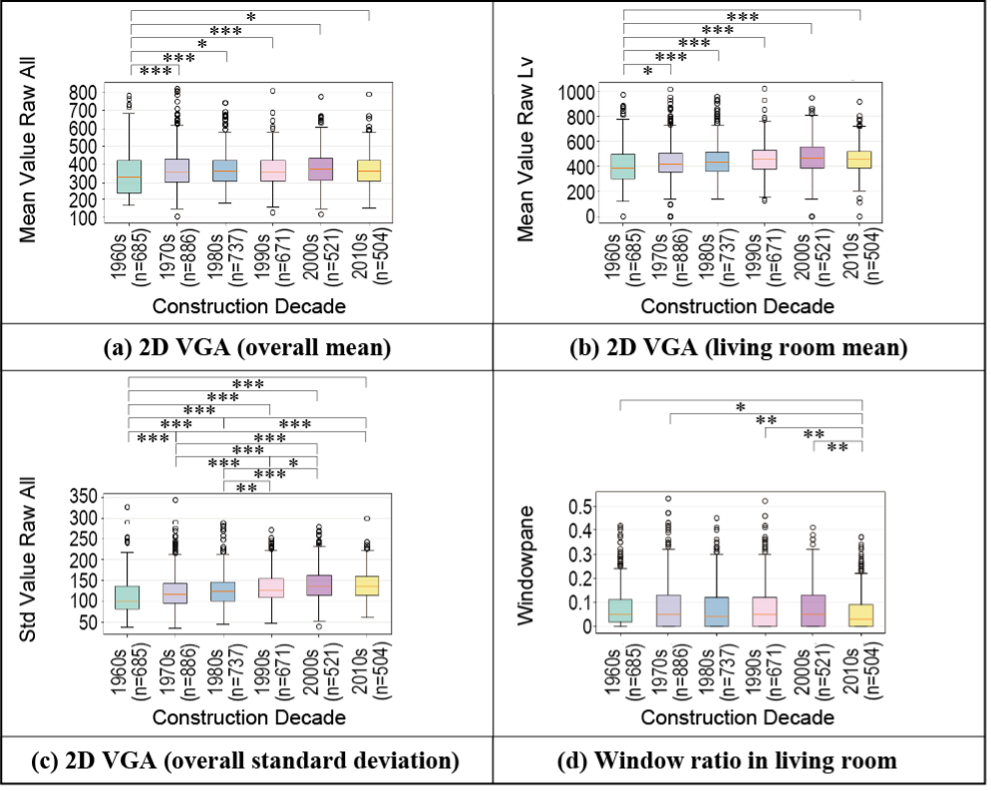
\includegraphics[width=0.95\textwidth]{chapters/plots/oneway.png}
    \caption{Temporal trends of openness indicators by construction decade showing (a) 2D openness scores for entire house, (b) 2D visibility scores for living rooms, (c) Standard deviation of 2D openness, and (d) 3D openness indicators (ceiling and window proportions). (***: 0.1\%, **: 1\%, *:5\%, ***:10\%)}
    \label{fig:temporal_trends}
\end{figure}

Table \ref{tab:anova_results} summarizes the one-way ANOVA results for each openness indicator across 
construction decades. The indicators show whether there are statistically significant differences between decades.

\begin{table}[htbp]
    \centering
    \begin{tabular}{l|c|c|c|c|c}
    \hline
    \textbf{Indicator} & \textbf{F-statistic} & \textbf{P-value} & \textbf{Significance} & \textbf{$\eta^2$} & \textbf{Effect Size} \\
    \hline
    Overall mean & 5.87 & 0.000021 & Yes & 0.0073 & Very small \\
    Living room mean & 17.15 & 0.000000 & Yes & 0.0210 & Small \\
    Overall std & 51.86 & 0.000000 & Yes & 0.0609 & Medium \\
    Window ratio & 3.63 & 0.002832 & Yes & 0.0045 & Very small \\
    \hline
    \end{tabular}
    \caption{One-way ANOVA results for openness indicators across construction decades (n=4,004, 6 groups analyzed).}
    \label{tab:anova_results}
\end{table}

The temporal effect is observed in the overall standard deviation of openness ($ \eta^2 = 0.0609$, medium effect), indicating 
that the variation in spatial layout within properties has changed substantially over time. 
Living room mean openness shows a small but notable effect ($ \eta^2 = 0.0210$), while overall mean openness and window ratio demonstrate very small effects despite statistical significance.
To understand the temporal changes of each indicator, the following sections discuss the results of each indicator in more detail.

\subsection{Pairwise Analysis of Temporal Changes for Each Indicator}

We conducted Tukey's HSD 
post-hoc tests for these indicators. This analysis reveals which specific decades differ 
significantly from each other and helps identify the direction and magnitude of changes over time.

\subsubsection{Mean visibility value of whole property}
\begin{table}[htbp]
    \centering
    \begin{tabular}{l|c|c|c|c|c|c}
    \hline
    \textbf{Comparison} & \textbf{Mean Diff.} & \textbf{\% Diff.} & \textbf{Cohen's d} & \textbf{Effect Size} & \textbf{P-value} & \textbf{Sig.} \\
    \hline
    1960s vs 1970s & -24.39 & -6.49\% & -0.2139 & Small & 0.0000 & Yes \\
    1960s vs 1980s & -21.33 & -5.73\% & -0.1930 & Negligible & 0.0007 & Yes \\
    1960s vs 1990s & -18.03 & -4.88\% & -0.1663 & Negligible & 0.0107 & Yes \\
    1960s vs 2000s & -24.53 & -6.53\% & -0.2159 & Small & 0.0003 & Yes \\
    1960s vs 2010s & -19.00 & -5.13\% & -0.1705 & Negligible & 0.0141 & Yes \\
    1970s vs 1980s & +3.06 & +0.82\% & +0.0313 & Negligible & 0.9897 & No \\
    1970s vs 1990s & +6.36 & +1.72\% & +0.0670 & Negligible & 0.8107 & No \\
    1970s vs 2000s & -0.14 & -0.04\% & -0.0014 & Negligible & 1.0000 & No \\
    1970s vs 2010s & +5.39 & +1.46\% & +0.0560 & Negligible & 0.9264 & No \\
    1980s vs 1990s & +3.30 & +0.89\% & +0.0374 & Negligible & 0.9893 & No \\
    1980s vs 2000s & -3.20 & -0.85\% & -0.0349 & Negligible & 0.9933 & No \\
    1980s vs 2010s & +2.33 & +0.63\% & +0.0262 & Negligible & 0.9986 & No \\
    1990s vs 2000s & -6.50 & -1.73\% & -0.0741 & Negligible & 0.8725 & No \\
    1990s vs 2010s & -0.97 & -0.26\% & -0.0115 & Negligible & 1.0000 & No \\
    2000s vs 2010s & +5.53 & +1.49\% & +0.0626 & Negligible & 0.9485 & No \\
    \hline
    \end{tabular}
    \caption{Pairwise comparisons (Tukey HSD) for mean visibility value of whole property across construction decades, showing mean differences, effect sizes, and statistical significance.}
    \label{tab:mean_vga_tukey_hsd}
\end{table}

As shown in Table \ref{tab:mean_vga_tukey_hsd}, this pattern reveals a clear temporal discontinuity: the 1960s properties demonstrate consistently higher 
mean visibility values with differences ranging from 4.88\% to 6.53\% compared to all subsequent decades. The 
effect sizes are generally small to negligible, but the consistent direction of differences suggests a 
meaningful architectural shift. After the 1970s, spatial openness characteristics remained roughly 
stable, with all pairwise differences being non-significant. This suggests 
that the significant shift in spatial design philosophy occurred between the 1960s and 1970s, likely 
reflecting the transition from post-war reconstruction architectural practices to more standardized 
residential design approaches that have persisted through the 2010s.

\subsubsection{Mean visibility value of living room}
\begin{table}[htbp]
    \centering
    \begin{tabular}{l|c|c|c|c|c|c}
    \hline
    \textbf{Comparison} & \textbf{Mean Diff.} & \textbf{\% Diff.} & \textbf{Cohen's d} & \textbf{Effect Size} & \textbf{P-value} & \textbf{Sig.} \\
    \hline
    1960s vs 1970s & -18.79 & -4.37\% & -0.1344 & Negligible & 0.0400 & Yes \\
    1960s vs 1980s & -31.80 & -7.18\% & -0.2350 & Small & 0.0000 & Yes \\
    1960s vs 1990s & -46.57 & -10.18\% & -0.3495 & Small & 0.0000 & Yes \\
    1960s vs 2000s & -54.53 & -11.72\% & -0.3888 & Small & 0.0000 & Yes \\
    1960s vs 2010s & -46.48 & -10.16\% & -0.3477 & Small & 0.0000 & Yes \\
    1970s vs 1980s & -13.01 & -2.94\% & -0.1035 & Negligible & 0.3031 & No \\
    1970s vs 1990s & -27.79 & -6.07\% & -0.2252 & Small & 0.0002 & Yes \\
    1970s vs 2000s & -35.74 & -7.68\% & -0.2775 & Small & 0.0000 & Yes \\
    1970s vs 2010s & -27.70 & -6.05\% & -0.2261 & Small & 0.0012 & Yes \\
    1980s vs 1990s & -14.77 & -3.23\% & -0.1270 & Negligible & 0.2396 & No \\
    1980s vs 2000s & -22.73 & -4.88\% & -0.1865 & Negligible & 0.0204 & Yes \\
    1980s vs 2010s & -14.68 & -3.21\% & -0.1285 & Negligible & 0.3337 & No \\
    1990s vs 2000s & -7.96 & -1.71\% & -0.0672 & Negligible & 0.8890 & No \\
    1990s vs 2010s & +0.09 & +0.02\% & +0.0008 & Negligible & 1.0000 & No \\
    2000s vs 2010s & +8.05 & +1.76\% & +0.0691 & Negligible & 0.9108 & No \\
    \hline
    \end{tabular}
    \caption{Pairwise comparisons (Tukey HSD) for mean visibility value of living room across construction decades, showing mean differences, effect sizes, and statistical significance.}
    \label{tab:living_room_vga_tukey_hsd}
\end{table}

As shown in Table \ref{tab:living_room_vga_tukey_hsd}, the analysis reveals a clear temporal trend in living room openness: properties built in the 1960s 
consistently demonstrate higher visibility values compared to all subsequent decades, with differences 
from 4.37\% (vs. 1970s) to 11.72\% (vs. 2000s). This decline shows a progressive pattern through the 
1980s, 1990s, and 2000s, with effect sizes increasing from negligible to small. Notably, the 2010s 
show no significant difference from the 1990s, suggesting a stabilization of living room design 
characteristics since the 1990s. The 1970s properties show significantly lower openness compared to 
later decades (1990s, 2000s, 2010s), while the 1980s only differ significantly from the 2000s. This 
pattern suggests that living room design became progressively more compartmentalized from the 1960s 
through the 2000s, potentially reflecting changing privacy preferences, space optimization strategies, 
or regulatory changes in residential architecture.

\subsubsection{Standard deviation of visibility values of whole property}
\begin{table}[htbp]
    \centering
    \begin{tabular}{l|c|c|c|c|c|c}
    \hline
    \textbf{Comparison} & \textbf{Mean Diff.} & \textbf{\% Diff.} & \textbf{Cohen's d} & \textbf{Effect Size} & \textbf{P-value} & \textbf{Sig.} \\
    \hline
    1960s vs 1970s & -8.70 & -7.21\% & -0.2204 & Small & 0.0001 & Yes \\
    1960s vs 1980s & -13.77 & -10.95\% & -0.3556 & Small & 0.0000 & Yes \\
    1960s vs 1990s & -20.88 & -15.71\% & -0.5382 & Medium & 0.0000 & Yes \\
    1960s vs 2000s & -27.17 & -19.52\% & -0.6740 & Medium & 0.0000 & Yes \\
    1960s vs 2010s & -26.18 & -18.94\% & -0.6851 & Medium & 0.0000 & Yes \\
    1970s vs 1980s & -5.07 & -4.03\% & -0.1392 & Negligible & 0.0654 & No \\
    1970s vs 1990s & -12.17 & -9.16\% & -0.3347 & Small & 0.0000 & Yes \\
    1970s vs 2000s & -18.47 & -13.27\% & -0.4924 & Small & 0.0000 & Yes \\
    1970s vs 2010s & -17.47 & -12.64\% & -0.4917 & Small & 0.0000 & Yes \\
    1980s vs 1990s & -7.11 & -5.35\% & -0.2019 & Small & 0.0043 & Yes \\
    1980s vs 2000s & -13.40 & -9.63\% & -0.3686 & Small & 0.0000 & Yes \\
    1980s vs 2010s & -12.41 & -8.98\% & -0.3644 & Small & 0.0000 & Yes \\
    1990s vs 2000s & -6.30 & -4.52\% & -0.1734 & Negligible & 0.0411 & Yes \\
    1990s vs 2010s & -5.30 & -3.83\% & -0.1566 & Negligible & 0.1444 & No \\
    2000s vs 2010s & +1.00 & +0.72\% & +0.0283 & Negligible & 0.9981 & No \\
    \hline
    \end{tabular}
    \caption{Pairwise comparisons (Tukey HSD) for standard deviation of visibility values of whole property across construction decades, showing mean differences, effect sizes, and statistical significance.}
    \label{tab:std_vga_tukey_hsd}
\end{table}

As shown in Table \ref{tab:std_vga_tukey_hsd}, the analysis reveals a strong temporal trend in spatial variability: properties built in the 1960s 
consistently show higher standard deviation of visibility values compared to all subsequent decades, with differences 
ranging from 7.21\% (vs. 1970s) to 19.52\% (vs. 2000s). This decline indicates a progressive 
reduction in spatial diversity within properties, suggesting that modern residential designs 
feature more functionally specialized rooms with reduced visual accessibility due to more detailed room design. 
The effect sizes progressively increase from small (1970s-1980s comparisons) to medium 
(1990s onwards comparisons with 1960s), indicating that this spatial compartmentalization became 
more pronounced over time. Notably, the 1990s and 2010s show no significant difference, and the 
2000s and 2010s are virtually identical, suggesting that spatial compartmentalization reached a 
plateau by the 1990s. This pattern likely reflects the evolution toward more compartmentalized 
floor plans with increased room specialization, where living areas, bedrooms, and other functional 
spaces became more clearly delineated and visually separated, contrasting with the more spatially 
integrated and varied arrangements characteristic of 1960s housing.

\subsubsection{Window Ratio}
\begin{table}[htbp]
    \centering
    \begin{tabular}{l|c|c|c|c|c|c}
    \hline
    \textbf{Comparison} & \textbf{Mean Diff.} & \textbf{\% Diff.} & \textbf{Cohen's d} & \textbf{Effect Size} & \textbf{P-value} & \textbf{Sig.} \\
    \hline
    1960s vs 1970s & -0.0017 & -2.06\% & -0.0189 & Negligible & 0.9991 & No \\
    1960s vs 1980s & +0.0055 & +7.49\% & +0.0652 & Negligible & 0.8472 & No \\
    1960s vs 1990s & +0.0017 & +2.19\% & +0.0195 & Negligible & 0.9993 & No \\
    1960s vs 2000s & -0.0023 & -2.84\% & -0.0273 & Negligible & 0.9977 & No \\
    1960s vs 2010s & +0.0166 & +26.84\% & +0.2104 & Small & 0.0155 & Yes \\
    1970s vs 1980s & +0.0071 & +9.76\% & +0.0785 & Negligible & 0.5757 & No \\
    1970s vs 1990s & +0.0033 & +4.34\% & +0.0359 & Negligible & 0.9761 & No \\
    1970s vs 2000s & -0.0006 & -0.79\% & -0.0069 & Negligible & 1.0000 & No \\
    1970s vs 2010s & +0.0183 & +29.51\% & +0.2075 & Small & 0.0025 & Yes \\
    1980s vs 1990s & -0.0038 & -4.93\% & -0.0422 & Negligible & 0.9655 & No \\
    1980s vs 2000s & -0.0078 & -9.61\% & -0.0880 & Negligible & 0.6312 & No \\
    1980s vs 2010s & +0.0111 & +18.00\% & +0.1330 & Negligible & 0.2362 & No \\
    1990s vs 2000s & -0.0040 & -4.92\% & -0.0437 & Negligible & 0.9712 & No \\
    1990s vs 2010s & +0.0149 & +24.12\% & +0.1729 & Negligible & 0.0441 & Yes \\
    2000s vs 2010s & +0.0189 & +30.54\% & +0.2257 & Small & 0.0072 & Yes \\
    \hline
    \end{tabular}
    \caption{Pairwise comparisons (Tukey HSD) for window ratio across construction decades, showing mean differences, effect sizes, and statistical significance.}
    \label{tab:window_tukey_hsd}
\end{table}

As shown in Table \ref{tab:window_tukey_hsd}, the post-hoc analysis reveals a clear temporal pattern: the 2010s properties show significantly higher window ratios 
compared to the 1960s, 1970s, 1990s, and 2000s, with effect sizes ranging from negligible to small. The 2010s demonstrate 
the highest window proportions, with increases of 26.84\% compared to the 1960s, 29.51\% compared to the 1970s, 24.12\% 
compared to the 1990s, and 30.54\% compared to the 2000s. This increase in window proportions in recent constructions 
likely reflects modern design preferences emphasizing natural light, improved construction technologies allowing for 
larger window installations, and changing lifestyle preferences that value bright, well-lit living spaces. This trend may also reflect 
advances in window technology, improved insulation materials, and energy-efficient glass that make larger windows 
more practical from both comfort and energy efficiency perspectives.

\section{Geospatial Distribution of Openness Indicators}

Figure \ref{fig:geospatial_distribution} shows the geospatial distribution of representative openness indicators in Tokyo's 23 wards.
Of the 4,004 properties analyzed, 
approximately 3,800 properties with postal code-level address information were selected for 
geospatial analysis. Here, we discuss the results obtained using a spatial interpolation method called 
kriging.

\begin{figure}[htbp]
    \centering
    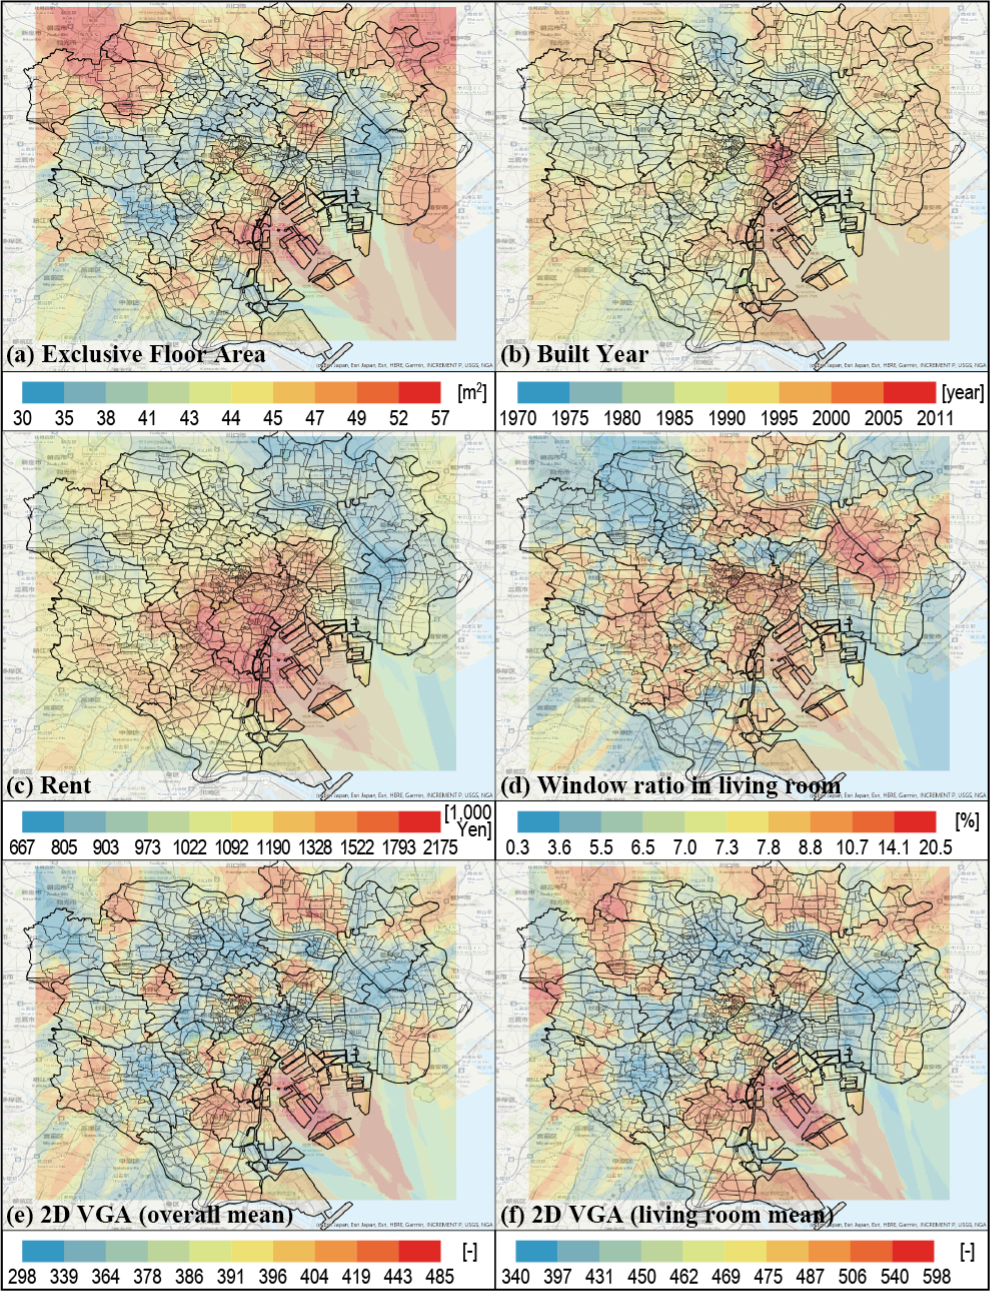
\includegraphics[width=0.95\textwidth]{chapters/plots/gis.png}
    \caption{Geospatial distribution maps showing: (a) Property rent levels, (b) Construction year distribution, (c) Floor area patterns, (d) Living room window ratios, (e) 2D openness for living rooms, and (f) 2D openness for entire houses.}
    \label{fig:geospatial_distribution}
\end{figure}

The spatial patterns of openness represented by overall and living room mean visibility values, 
rent, construction year, and floor area are partially correlated, 
indicating that urban redevelopment and housing design trends are manifesting geographically. This 
correlation suggests that certain areas of Tokyo have experienced similar development and 
design philosophies.

The ratio of living room windows tends to be high in center areas  (6d). This pattern is 
possible to be influenced by the existence of high-rise apartments where views are valued. In central 
Tokyo, the premium on natural light and city views drives building constructors to increase the window space, 
especially in living rooms where residents spend most of their waking hours. The emphasis on windows 
in these areas also reflects the higher property values that can justify the additional costs of 
better views.

Areas with high visibility values are scattered throughout the southern part of the city center and 
other areas (6e and 6f). This scattered distribution suggests that open floor plans are not 
concentrated in any single district but rather reflect various factors including development timing, 
target demographics, and local planning regulations. The southern areas may benefit from better 
sunlight exposure, making open layouts more attractive and practical.

The relatively low visibility values in suburban areas are thought to be influenced by housing types 
with many individual rooms and housing complexes. Suburban housing often reflects traditional 
Japanese housing preferences that prioritize privacy and clearly defined spaces for different 
activities. These areas may also have more families with children, where separated rooms serve 
practical purposes for study, sleep, and family activities.

\section{Correlation Analysis Among Indicators and with Rent and Others}

Figure \ref{fig:corr_plots} shows the correlation between 2D/3D openness indicators,  between openness indicators and 
rent,  along with other indicators. This analysis helps us understand how different aspects of spatial openness 
relate to each other and to market factors.

\begin{figure}[htbp]
    \centering
    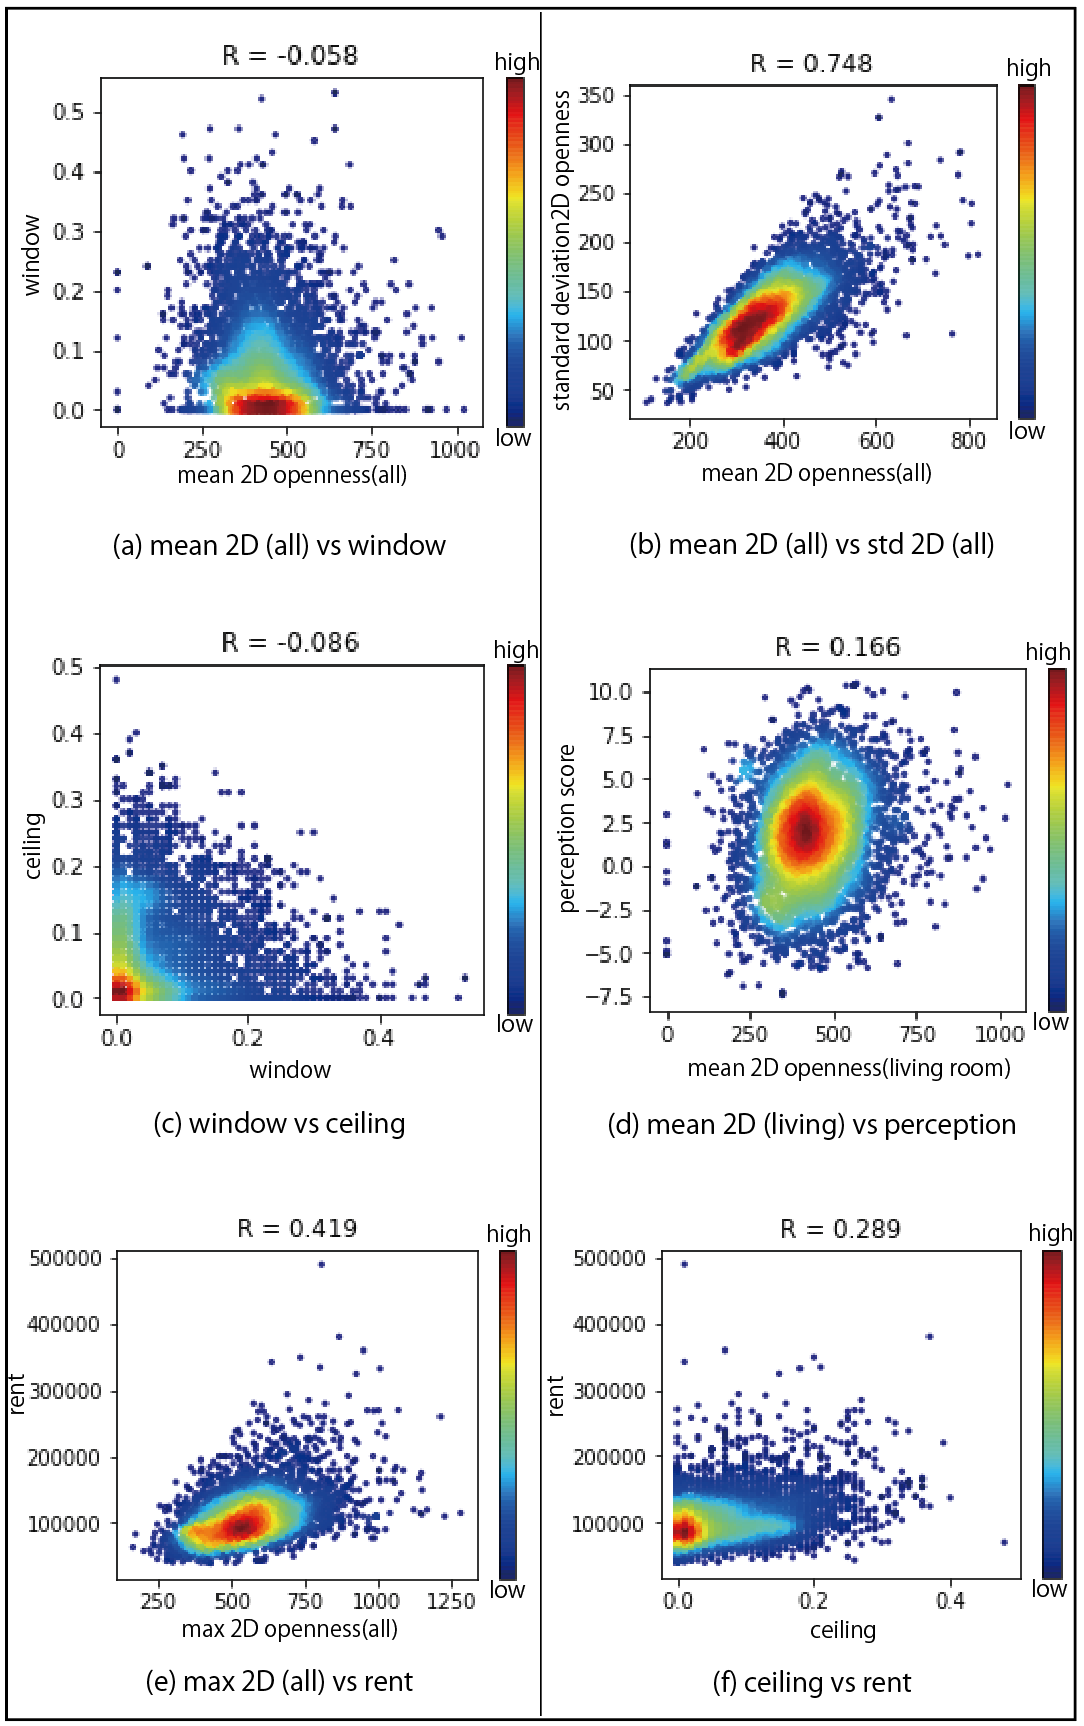
\includegraphics[width=0.8\textwidth]{chapters/plots/corr_plots.png}
    \caption{Correlation analysis showing: (a) 2D vs 3D openness indicators, (b) Mean vs standard deviation of 2D openness, (c) Relationships among 3D openness indicators, (d) 2D openness vs impression evaluation scores, and (e) Openness indicators vs rent levels.}
    \label{fig:corr_plots}
\end{figure}

No clear correlation was found between the 2D openness indicator and the 3D openness indicator, namely the window ratio VS.
the mean visibility value of the properties (7a). This finding suggests that floor plan openness and vertical spatial characteristics 
operate independently in residential design. A house might have an open floor plan but low window ratio, 
or conversely, have separated rooms but high ceilings and large windows. This independence indicates 
that designers and residents can achieve different types of openness through various design 
strategies.

On the other hand, a high correlation was confirmed between the mean value and standard deviation of 
2D openness (7b). This relationship indicates that properties with higher average 2D openness 
also tend to have greater variation in openness across different spaces. This pattern makes sense 
from a design perspective, as houses with very open living areas often offers larger area and maintain more functionality focused, 
enclosed spaces for perhaps multiple bedrooms and bathrooms, creating a higher deivations in visibility values between small rooms
and large rooms.

The 3D openness indicators were generally complementary to each other (7c). This 
complementary relationship suggests that different vertical spatial elements work together to create 
the overall sense of openness in interior spaces. For example, rooms with smaller windows might 
compensate with higher ceilings or more visible ceiling area to maintain a sense of spaciousness.

Additionally, there was a tendency for properties with higher openness to have higher rent price (7e). 
This positive correlation indicates that spatial openness is valued in the rental market and 
commands a premium. Tenants appear willing to pay more for properties that offer better visual 
connectivity, more natural light, and a greater sense of space. This market preference validates the 
importance of openness as a design consideration for rental properties.

Here in (d), we introduce a impression evaluation score that presents the user perception goodness from one of the 
previous research in our lab, which utilizes a trained feature extraction network to extract 1D feature 
vector from interior images, then input to a preference scoring model that was trained over a set of user annotated dataset. 
The detailed information can refer to this report \cite{oki2023rental}. With these impression evaluation scores calculated for all 4,004 
properties, we can also investigate the correlation between these scores and 2D openness indicators for living rooms. 
Comparing these scores with 2D openness indicators for living rooms, there was almost no correlation between them (7d), showing
the clear perception gap between a 2D floorplan image and the actual living room photograph to users' eyes. 

While spatial openness is one of the elements that characterize a space, this result suggests that 
other elements such as interior design and furniture may have a greater influence on impressions. The 
lack of correlation between objective openness measures and subjective impressions reveals the 
complexity of how people perceive and evaluate living spaces. Factors such as color schemes, lighting 
quality, furniture style and arrangement, cleanliness, and overall aesthetic appeal may play more 
significant roles in forming positive impressions than the geometric properties of the space itself.

% This finding has important implications for both researchers and practitioners in housing design. 
% While objective measures of openness provide valuable insights into spatial characteristics, they may 
% not fully capture the human experience of living in these spaces. Future research should consider 
% incorporating more subjective measures and qualitative factors to develop a more complete 
% understanding of residential space quality and user satisfaction.



\section{Impact of Openness Indicators on Rental Prices}

To further investigate the relationship between openness indicators and market value, we developed 
multivariate linear regression models to fit the rental prices using the various openness indicators. 
This analysis aims to quantify the economic impact of spatial openness characteristics and identify 
which specific indicators contribute most significantly to rental price determination.

\subsubsection{Fitting with Unselected Features }
The predictive modeling process involved selecting relevant features from our comprehensive set of 
openness indicators. Table \ref{tab:selected_features} presents the features for the 
regression model, categorized by their measurement type and spatial scope.

\begin{table}[htbp]
    \centering
    \begin{tabular}{l|l|l}
    \hline
    \textbf{Category} & \textbf{Feature} & \textbf{Description} \\
    \hline
    \multirow{4}{*}{Whole Property 2D} & min\_value\_raw\_all & Minimum visibility value across all spaces \\
     & max\_value\_raw\_all & Maximum visibility value across all spaces \\
     & mean\_value\_raw\_all & Average visibility value across all spaces \\
     & std\_value\_raw\_all & Standard deviation of visibility values \\
    \hline
    \multirow{4}{*}{Living Room 2D} & mean\_value\_raw\_lv & Average visibility value in living room \\
     & min\_value\_raw\_lv & Minimum visibility value in living room \\
     & max\_value\_raw\_lv & Maximum visibility value in living room \\
     & std\_value\_raw\_lv & Standard deviation of visibility in living room \\
    \hline
    \multirow{4}{*}{3D Openness} & windowpane & Proportion of window area \\
     & floor & Proportion of visible floor area \\
     & ceiling & Proportion of visible ceiling area \\
     & wall & Proportion of visible wall area \\
    \hline
    \end{tabular}
    \caption{Selected features for rental price prediction model, organized by measurement category and spatial scope.}
    \label{tab:selected_features}
\end{table}

After performing the initial regression fit using these features, 
we obtained the regression results shown in Figure \ref{fig:feature_R2_red}. 
The model achieved an R² of 0.3, indicating moderate predictive power in explaining rental price variance through our openness indicators. 
Residual analysis revealed no clear imbalance in the error distribution, suggesting negligible bias in the linear model fit. 
The results illustrate the predictive performance and feature importance of our openness indicators 
for rental price prediction.

\begin{figure}[htbp]
    \centering
    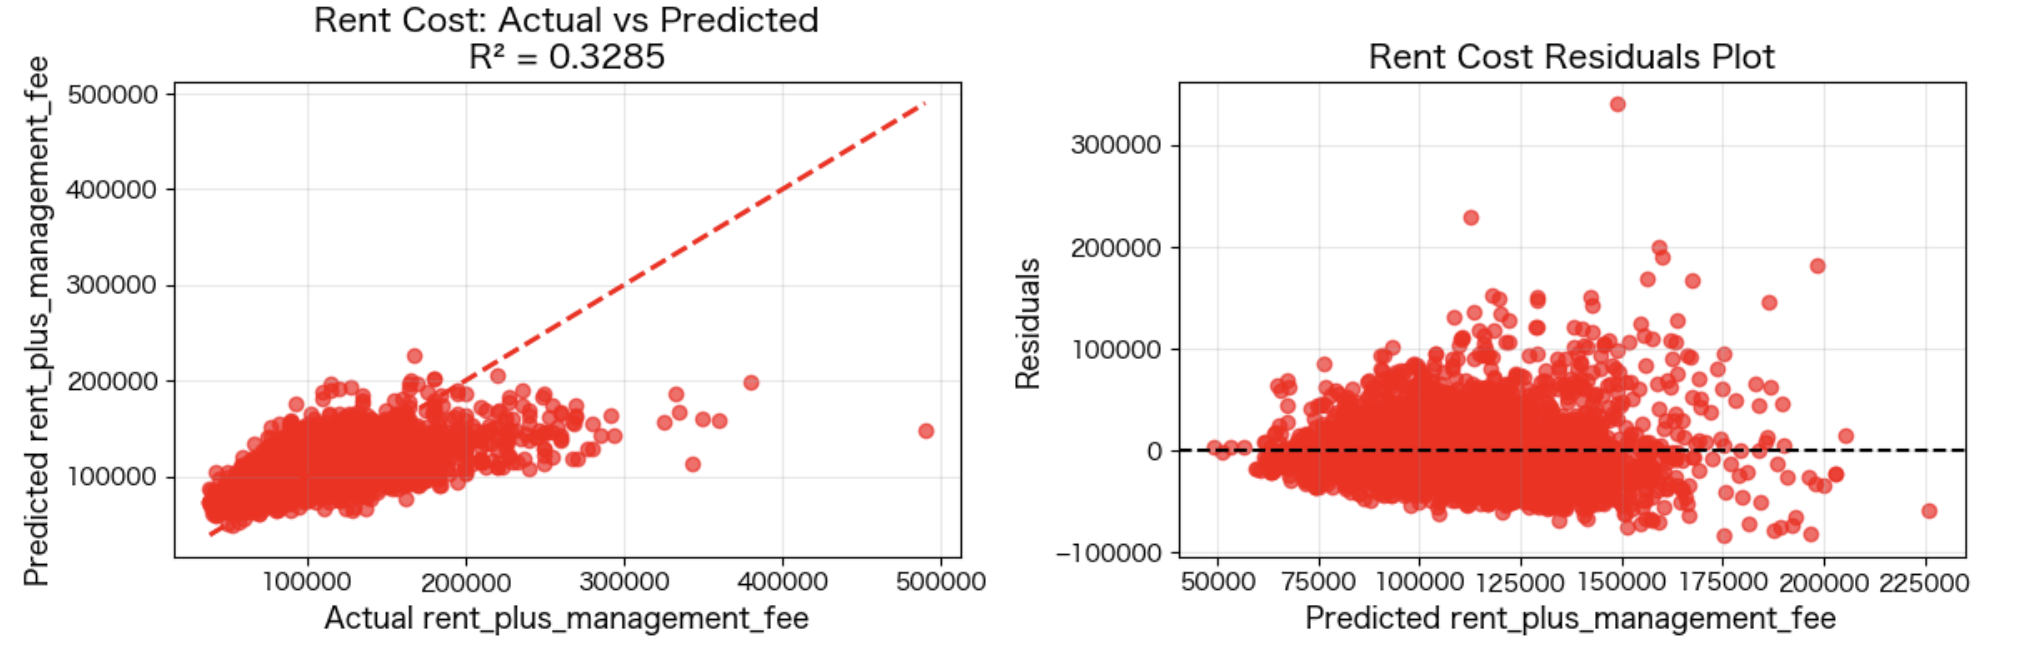
\includegraphics[width=0.95\textwidth]{chapters/plots/12_feature_R2_red.png}
    \caption{Predictive performance and feature importance analysis for rental price prediction using openness indicators. The figure shows R² scores and relative importance rankings of different spatial openness measures in determining rental prices.}
    \label{fig:feature_R2_red}
\end{figure}


\subsubsection{Correlation and VIF Checks to Reduce Multicollinearity}
The correlations within the features is displayed in Figure \ref{fig:12_feature_corr}, and the feature 
importance is displayed in Figure \ref{fig:12_feature_imp}.

\begin{figure}[htbp]
    \centering
    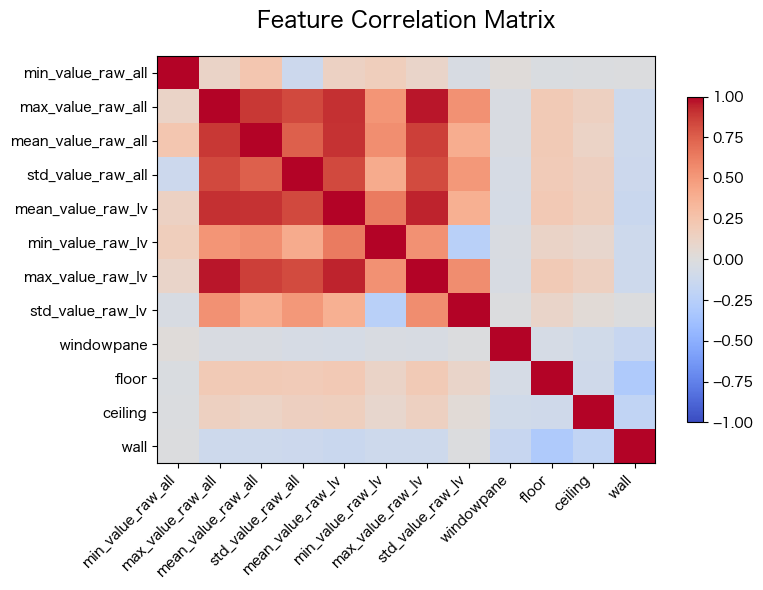
\includegraphics[width=0.95\textwidth]{chapters/plots/12_feature_corr.png}
    \caption{Predictive performance of openness indicators for rental price prediction showing R² scores and feature importance rankings. The model demonstrates the relative contribution of different spatial openness measures to rental price determination.}
    \label{fig:12_feature_corr}
\end{figure}
\begin{figure}[htbp]
    \centering
    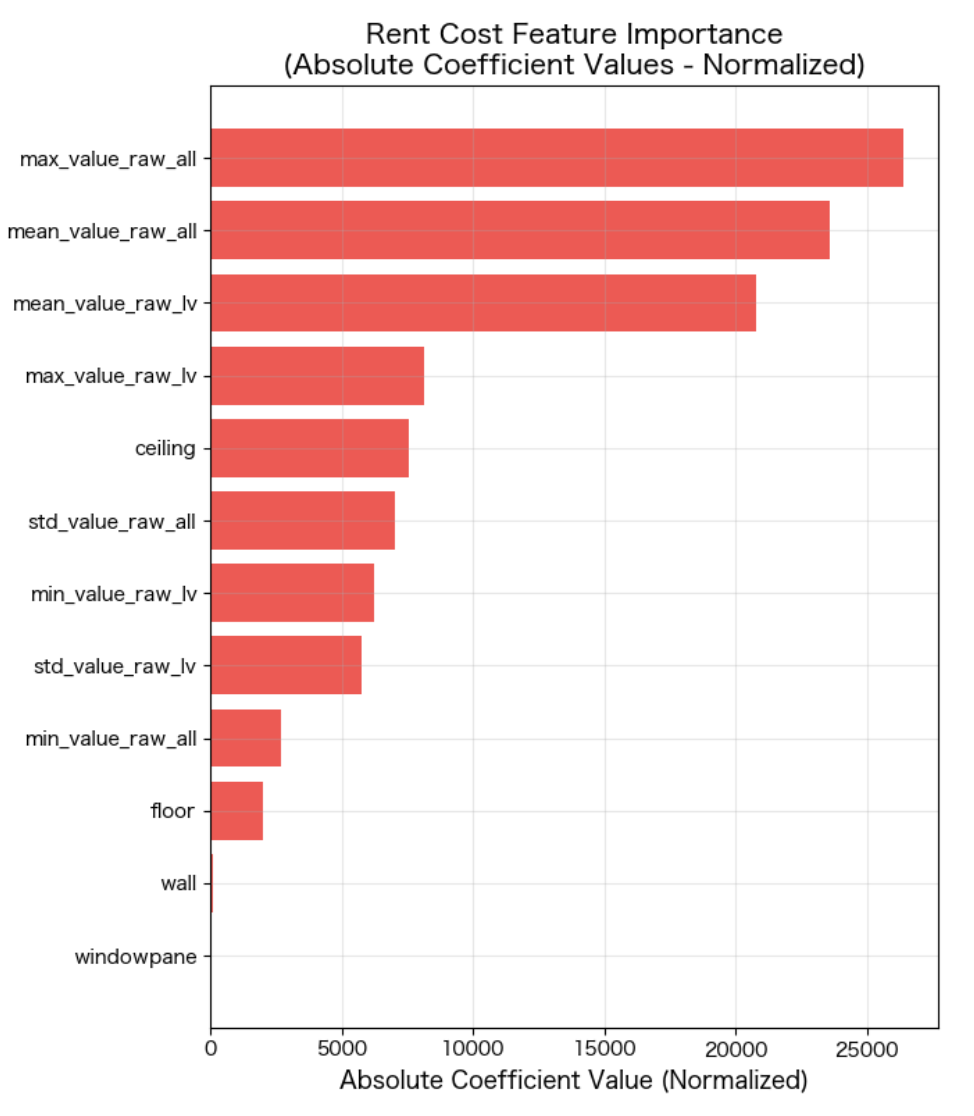
\includegraphics[width=0.6\textwidth]{chapters/plots/12_feature_imp.png}
    \caption{Correlation matrix and feature importance analysis for the 12 selected openness indicators used in rental price prediction. The heatmap shows inter-feature correlations while the importance scores indicate each feature's contribution to the predictive model.}
    \label{fig:12_feature_imp}
\end{figure}

To address potential multicollinearity issues observed in the feature correlation analysis, we conducted 
Variance Inflation Factor (VIF) checks and employed stepwise feature selection to identify the optimal 
feature subset while maintaining model performance. High correlation between certain features suggested 
redundancy that could be eliminated without significant loss in predictive power.

The VIF analysis revealed several features with high multicollinearity ($VIF > 5$), particularly among 
the 2D openness measures within the same spatial scope, as shown in Table \ref{tab:vif_analysis}.
\begin{center}
    \begin{tabular}{l|c|l}
    \hline
    Feature & VIF & Status \\
    \hline
    \textcolor{red}{min\_value\_raw\_all} & 1.35 & Low \\
    \textcolor{red}{max\_value\_raw\_all} & 28.16 & High \\
    \textcolor{red}{mean\_value\_raw\_all} & 8.34 & Moderate \\
    \textcolor{red}{std\_value\_raw\_all} & 5.58 & Moderate \\
    min\_value\_raw\_lv & 3.40 & Low \\
    max\_value\_raw\_lv & 37.94 & High \\
    \textcolor{red}{std\_value\_raw\_lv} & 3.63 & Low \\
    mean\_value\_raw\_lv & 18.29 & High \\
    windowpane & 1.06 & Low \\
    floor & 1.21 & Low \\
    \textcolor{red}{ceiling} & 1.13 & Low \\
    wall & 1.23 & Low \\
    \hline
    \end{tabular}
    \captionof{table}{Variance Inflation Factor (VIF) for multicollinearity assessment, $VIF > 10$: High,
    $VIF > 5$: Moderate,
    $VIF < 5$: Low}
    \label{tab:vif_analysis}
\end{center}

\subsubsection{Stepwise Feature Selection for Optimal Model}
Based on the VIF analysis results, we selected the 7 features highlighted in red in Table \ref{tab:vif_analysis} 
with acceptable multicollinearity levels ($VIF < 10$) for the final model. These selected features include: 
min\_value\_raw\_all, max\_value\_raw\_all, mean\_value\_raw\_all, std\_value\_raw\_all, std\_value\_raw\_lv, 
and ceiling. Notably, all the visibility-based openness indicators from whole properties 
(min\_value\_raw\_all, max\_value\_raw\_all, mean\_value\_raw\_all, std\_value\_raw\_all) were retained 
after the selection, demonstrating their independence from each other and their distinct contributions 
to model performance. This refined feature set eliminated the most problematic variables while 
maintaining strong predictive performance. The results of this 7-feature model are shown in 
Figure \ref{fig:7_feature_R2_red}, demonstrating that the reduced model maintains comparable 
performance. The updated feature importance is shown in Figure \ref{fig:7_feature_imp}.

\subsubsection{Interpretation of Feature Importance}
The overall visibility values of properties demonstrate high importance 
because they capture the complete spatial connectivity and accessibility patterns
which directly relates to the perceived spaciousness and flow that tenants value. In contrast, the 
living room-specific features show relatively low importance, perhaps due to their partial representation 
of the property's overall spatial quality. For 3D openness indicators, only ceiling shows relatively good importance, 
possibly due to its strong correlation with perceived vertical spaciousness. 
However, we must understand that rent price is a very complicated target to predict and is 
certainly not impacted solely by our selected features. Therefore, our observations can 
only serve as potential insights to link the relationship between price and our openness indicators, 
not aiming to comprehensively predict the rent price under any assumption.

\begin{figure}[htbp]
    \centering
    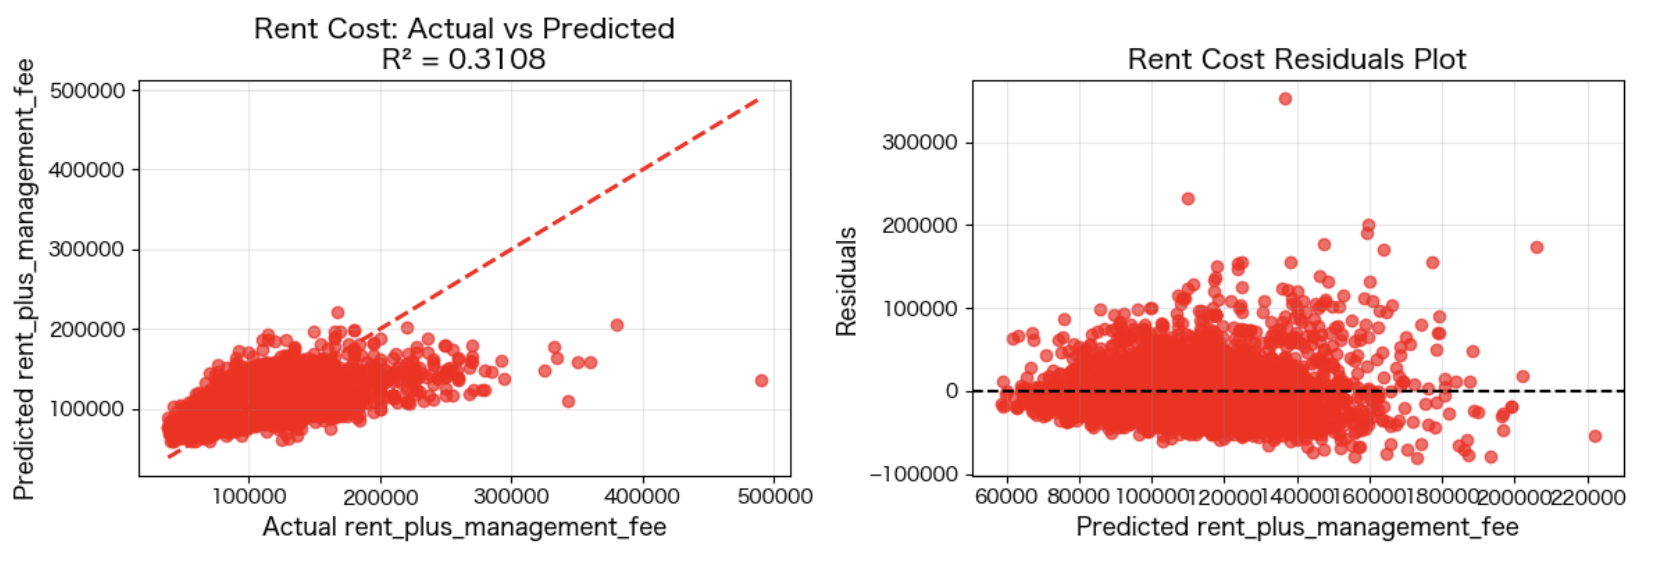
\includegraphics[width=0.95\textwidth]{chapters/plots/7_feature_R2_red.png}
    \caption{Predictive performance of with reduced features}
    \label{fig:7_feature_R2_red}
\end{figure}

\begin{figure}[htbp]
    \centering
    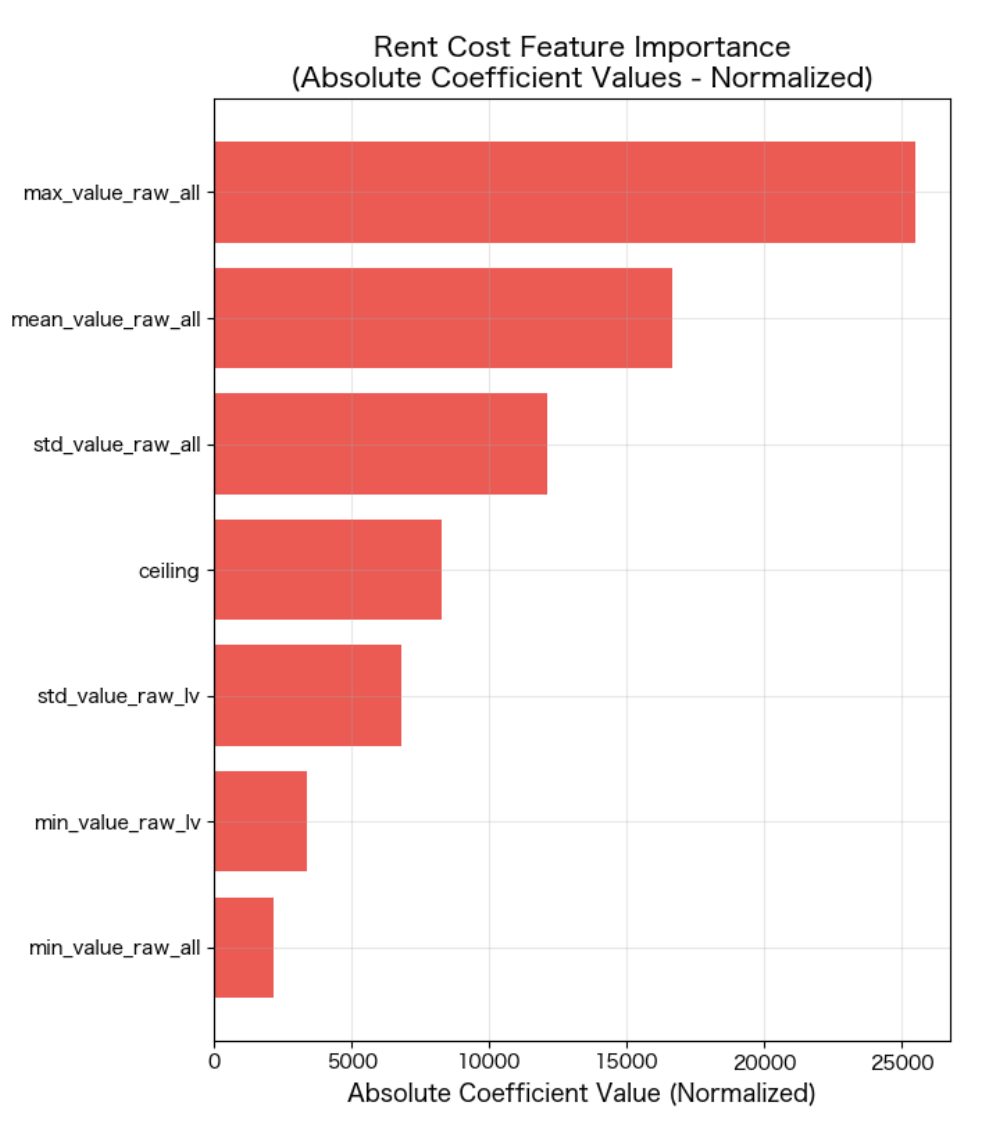
\includegraphics[width=0.6\textwidth]{chapters/plots/7_feature_imp.png}
    \caption{Feature importance of the 7 selected features}
    \label{fig:7_feature_imp}
\end{figure}



% \subsubsection{Statistical Test for Feature Impact on Rent Price}
% To better understand the impact of each feature on the rent price, we conducted a statistical test, with 
% null hypothesis that the feature has no impact on the rent price, and use t-Statistics to test the significance.
% The results are shown in Table \ref{tab:regression_coefficients}.
% \begin{center}
%     \begin{tabular}{l|c|c|c|c|c}
%     \hline
%     Feature & Coef. & Std & t-stat & p-value & Sig. \\
%      & ($\times 10^3$) & ($\times 10^2$) & & & \\
%     \hline
%     min\_all & -2.68 & 5.90 & -4.55 & 0.00 & Y \\
%     max\_all & 26.70 & 27.00 & 9.89 & 0.00 & Y \\
%     mean\_all & -23.80 & 14.70 & -16.19 & 0.00 & Y \\
%     std\_all & 6.77 & 12.00 & 5.64 & 0.00 & Y \\
%     min\_lv & -6.20 & 9.38 & -6.61 & 0.00 & Y \\
%     max\_lv & -4.08 & 31.30 & -1.30 & 0.19 & N \\
%     std\_lv & -7.97 & 9.69 & -8.23 & 0.00 & Y \\
%     median\_lv & 18.10 & 21.70 & 8.31 & 0.00 & Y \\
%     window & -0.07 & 5.24 & -0.14 & 0.89 & N \\
%     floor & -2.01 & 5.59 & -3.59 & 0.00 & Y \\
%     ceiling & 7.49 & 5.41 & 13.83 & 0.00 & Y \\
%     wall & -0.10 & 5.63 & -0.19 & 0.85 & N \\
%     \hline
%     \end{tabular}
%     \captionof{table}{Feature coefficients for rent prediction (normalized features), 
%     their t-stats and p-values in the test againest the impact towards the rent price. Confidence level set to 95\%.}
%     \label{tab:regression_coefficients}
% \end{center}


\section{Visual Validation of Openness Indicators}

To validate the reliability and interpretability of our openness indicators, we present a visual 
comparison of properties with varying openness characteristics. For each indicator, we collected 
properties from the top 25\% and bottom 25\% of the distribution, then sampled 2 properties 
from each group to showcase the intuitive impressions associated with different indicator values. 
This section simply showcases floor plans and corresponding living room images.
The visual examples demonstrate how the quantitative measures correspond to observable spatial 
characteristics, providing intuitive understanding of what the numerical indicators represent in 
actual residential spaces. This validation helps bridge the gap between computational analysis and 
human perception of spatial openness as an extra validation of the effectiveness of our methodolgies.

\subsection{2D Openness Indicators}

\subsubsection{Mean visibility values - Whole Property}

\begin{figure}[htbp]
    \centering
    \begin{subfigure}[b]{0.22\textwidth}
        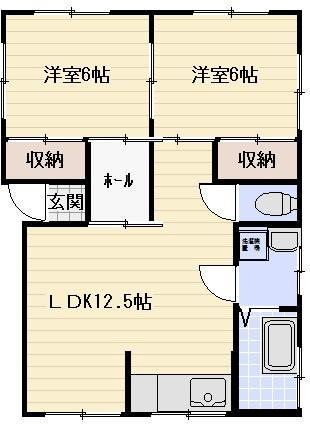
\includegraphics[width=\textwidth]{chapters/plots/ranked_properties/mean_value_raw_all/top_k/floorplan/1f_c8_24643c6e305738d8169422c2b5fa_0002.jpg}
        \caption*{High visibility - Floorplan 1}
    \end{subfigure}
    \begin{subfigure}[b]{0.22\textwidth}
        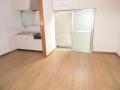
\includegraphics[width=\textwidth]{chapters/plots/ranked_properties/mean_value_raw_all/top_k/livingroom/1f_c8_24643c6e305738d8169422c2b5fa_0008.jpg}
        \caption*{High visibility - Living Room 1}
    \end{subfigure}
    \begin{subfigure}[b]{0.22\textwidth}
        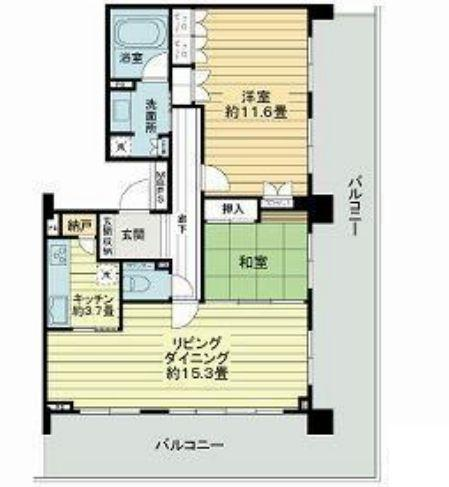
\includegraphics[width=\textwidth]{chapters/plots/ranked_properties/mean_value_raw_all/top_k/floorplan/64_4d_371f70a372a97ca79decb31c4d34_0001.jpg}
        \caption*{High visibility - Floorplan 2}
    \end{subfigure}
    \begin{subfigure}[b]{0.22\textwidth}
        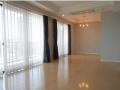
\includegraphics[width=\textwidth]{chapters/plots/ranked_properties/mean_value_raw_all/top_k/livingroom/64_4d_371f70a372a97ca79decb31c4d34_0003.jpg}
        \caption*{High visibility - Living Room 2}
    \end{subfigure}
    
    \begin{subfigure}[b]{0.22\textwidth}
        \includegraphics[width=\textwidth]{chapters/plots/ranked_properties/mean_value_raw_all/bottom_k/floorplan/0e_71_8cc2f7c9bdf62ed48ec31fe11dd8_0002.jpg}
        \caption*{Low visibility - Floorplan 1}
    \end{subfigure}
    \begin{subfigure}[b]{0.22\textwidth}
        \includegraphics[width=\textwidth]{chapters/plots/ranked_properties/mean_value_raw_all/bottom_k/livingroom/0e_71_8cc2f7c9bdf62ed48ec31fe11dd8_0005.jpg}
        \caption*{Low visibility - Living Room 1}
    \end{subfigure}
    \begin{subfigure}[b]{0.22\textwidth}
        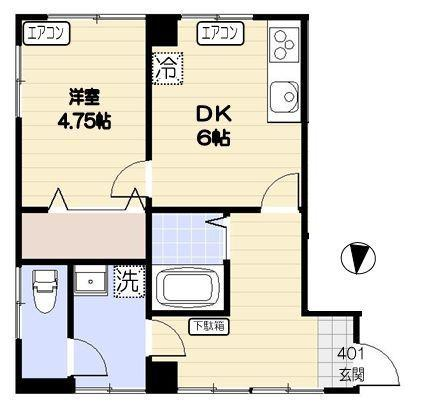
\includegraphics[width=\textwidth]{chapters/plots/ranked_properties/mean_value_raw_all/bottom_k/floorplan/5c_20_9ed0eaaf3e33292a6a0ab1a23b97_0003.jpg}
        \caption*{Low visibility - Floorplan 2}
    \end{subfigure}
    \begin{subfigure}[b]{0.22\textwidth}
        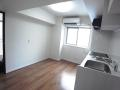
\includegraphics[width=\textwidth]{chapters/plots/ranked_properties/mean_value_raw_all/bottom_k/livingroom/5c_20_9ed0eaaf3e33292a6a0ab1a23b97_0002.jpg}
        \caption*{Low visibility - Living Room 2}
    \end{subfigure}
    \caption{Comparison of properties with high (top row) and low (bottom row) mean visibility values for entire property, showing both floor plans and corresponding living room images.}
    \label{fig:mean_vga_comparison}
\end{figure}

\subsubsection{Standard Deviation of visibility values}

\begin{figure}[htbp]
    \centering
    \begin{subfigure}[b]{0.22\textwidth}
        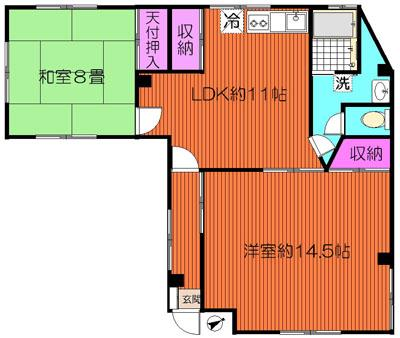
\includegraphics[width=\textwidth]{chapters/plots/ranked_properties/std_value_raw_all/top_k/floorplan/15_a7_04fb7626adc9839a2593d6cd4f42_0001.jpg}
        \caption*{High Std - Floorplan 1}
    \end{subfigure}
    \begin{subfigure}[b]{0.22\textwidth}
        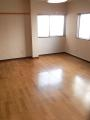
\includegraphics[width=\textwidth]{chapters/plots/ranked_properties/std_value_raw_all/top_k/livingroom/15_a7_04fb7626adc9839a2593d6cd4f42_0003.jpg}
        \caption*{High Std - Living Room 1}
    \end{subfigure}
    \begin{subfigure}[b]{0.22\textwidth}
        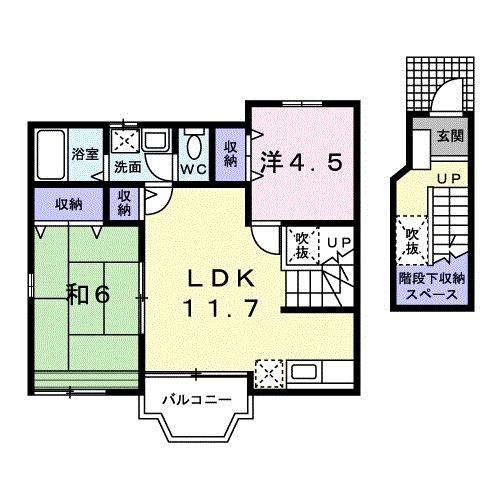
\includegraphics[width=\textwidth]{chapters/plots/ranked_properties/std_value_raw_all/top_k/floorplan/25_95_f67b75758ae45833a6b3146a5093_0002.jpg}
        \caption*{High Std - Floorplan 2}
    \end{subfigure}
    \begin{subfigure}[b]{0.22\textwidth}
        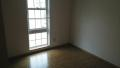
\includegraphics[width=\textwidth]{chapters/plots/ranked_properties/std_value_raw_all/top_k/livingroom/25_95_f67b75758ae45833a6b3146a5093_0010.jpg}
        \caption*{High Std - Living Room 2}
    \end{subfigure}
    
    \begin{subfigure}[b]{0.22\textwidth}
        \includegraphics[width=\textwidth]{chapters/plots/ranked_properties/std_value_raw_all/bottom_k/floorplan/0e_71_8cc2f7c9bdf62ed48ec31fe11dd8_0002.jpg}
        \caption*{Low Std - Floorplan 1}
    \end{subfigure}
    \begin{subfigure}[b]{0.22\textwidth}
        \includegraphics[width=\textwidth]{chapters/plots/ranked_properties/std_value_raw_all/bottom_k/livingroom/0e_71_8cc2f7c9bdf62ed48ec31fe11dd8_0005.jpg}
        \caption*{Low Std - Living Room 1}
    \end{subfigure}
    \begin{subfigure}[b]{0.22\textwidth}
        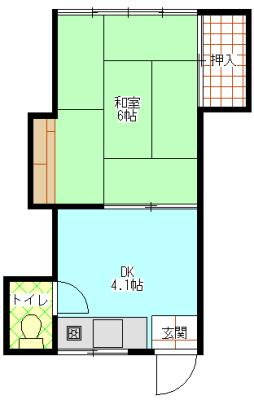
\includegraphics[width=\textwidth]{chapters/plots/ranked_properties/std_value_raw_all/bottom_k/floorplan/23_cf_c3504d142c310c319927e413f9b4_0002.jpg}
        \caption*{Low Std - Floorplan 2}
    \end{subfigure}
    \begin{subfigure}[b]{0.22\textwidth}
        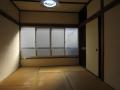
\includegraphics[width=\textwidth]{chapters/plots/ranked_properties/std_value_raw_all/bottom_k/livingroom/23_cf_c3504d142c310c319927e413f9b4_0003.jpg}
        \caption*{Low Std - Living Room 2}
    \end{subfigure}
    \caption{Comparison of properties with high (top row) and low (bottom row) standard deviation of visibility values, demonstrating spatial diversity within properties with both floor plans and corresponding living room images.}
    \label{fig:std_vga_comparison}
\end{figure}

\subsection{3D Openness Indicators}

\subsubsection{Window Ratio}

\begin{figure}[H]
    \centering
    \begin{subfigure}[b]{0.22\textwidth}
        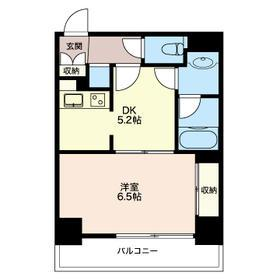
\includegraphics[width=\textwidth]{chapters/plots/ranked_properties/windowpane/top_k/floorplan/12_fc_ab7053681e787a077c7ac79a87cc_0001.jpg}
        \caption*{High Window - Floorplan 1}
    \end{subfigure}
    \begin{subfigure}[b]{0.22\textwidth}
        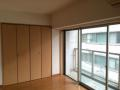
\includegraphics[width=\textwidth]{chapters/plots/ranked_properties/windowpane/top_k/livingroom/12_fc_ab7053681e787a077c7ac79a87cc_0004.jpg}
        \caption*{High Window - Living Room 1}
    \end{subfigure}
    \begin{subfigure}[b]{0.22\textwidth}
        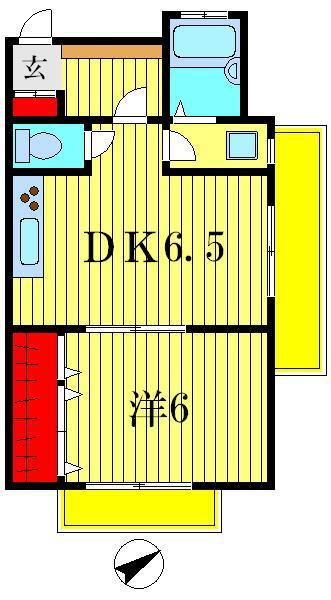
\includegraphics[width=\textwidth]{chapters/plots/ranked_properties/windowpane/top_k/floorplan/21_ce_5f9cc665f397a534afb3d328ba6e_0002.jpg}
        \caption*{High Window - Floorplan 2}
    \end{subfigure}
    \begin{subfigure}[b]{0.22\textwidth}
        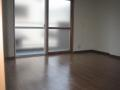
\includegraphics[width=\textwidth]{chapters/plots/ranked_properties/windowpane/top_k/livingroom/21_ce_5f9cc665f397a534afb3d328ba6e_0003.jpg}
        \caption*{High Window - Living Room 2}
    \end{subfigure}
    
    \begin{subfigure}[b]{0.22\textwidth}
        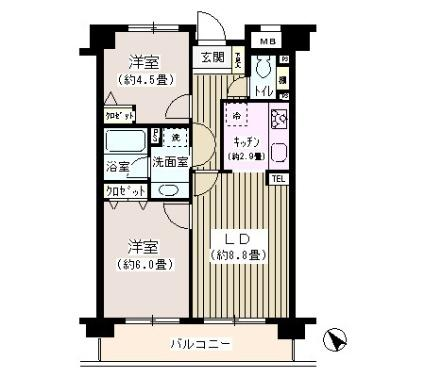
\includegraphics[width=\textwidth]{chapters/plots/ranked_properties/windowpane/bottom_k/floorplan/06_68_65ba9ef27b6ab9d58cfd41ec130c_0001.jpg}
        \caption*{Low Window - Floorplan 1}
    \end{subfigure}
    \begin{subfigure}[b]{0.22\textwidth}
        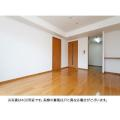
\includegraphics[width=\textwidth]{chapters/plots/ranked_properties/windowpane/bottom_k/livingroom/06_68_65ba9ef27b6ab9d58cfd41ec130c_0006.jpg}
        \caption*{Low Window - Living Room 1}
    \end{subfigure}
    \begin{subfigure}[b]{0.22\textwidth}
        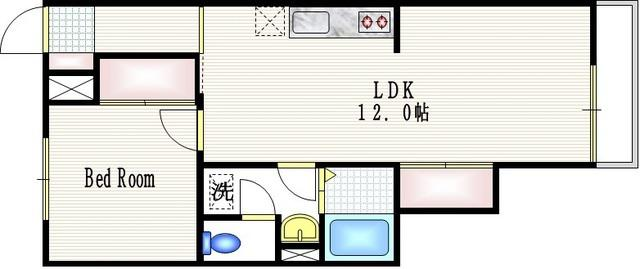
\includegraphics[width=\textwidth]{chapters/plots/ranked_properties/windowpane/bottom_k/floorplan/29_7a_1f51c95a1e83d18ff7977ee84a4f_0003.jpg}
        \caption*{Low Window - Floorplan 2}
    \end{subfigure}
    \begin{subfigure}[b]{0.22\textwidth}
        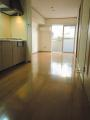
\includegraphics[width=\textwidth]{chapters/plots/ranked_properties/windowpane/bottom_k/livingroom/29_7a_1f51c95a1e83d18ff7977ee84a4f_0002.jpg}
        \caption*{Low Window - Living Room 2}
    \end{subfigure}
    \caption{Comparison of properties with high (top row) and low (bottom row) window ratios, showing the impact of glazing on interior brightness and openness perception with both floor plans and corresponding living room images.}
    \label{fig:windowpane_comparison}
\end{figure}

\subsubsection{Ceiling Visibility}

\begin{figure}[H]
    \centering
    \begin{subfigure}[b]{0.22\textwidth}
        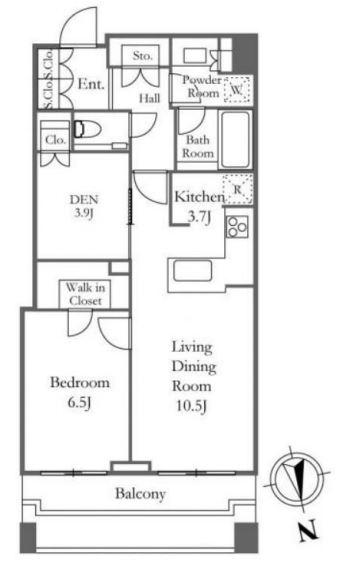
\includegraphics[width=\textwidth]{chapters/plots/ranked_properties/ceiling/top_k/floorplan/06_51_0b8ef8c9d9446fd1239774622f9f_0002.jpg}
        \caption*{High Ceiling - Floorplan 1}
    \end{subfigure}
    \begin{subfigure}[b]{0.22\textwidth}
        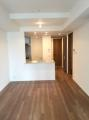
\includegraphics[width=\textwidth]{chapters/plots/ranked_properties/ceiling/top_k/livingroom/06_51_0b8ef8c9d9446fd1239774622f9f_0003.jpg}
        \caption*{High Ceiling - Living Room 1}
    \end{subfigure}
    \begin{subfigure}[b]{0.22\textwidth}
        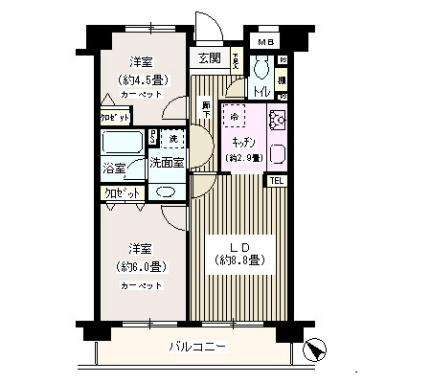
\includegraphics[width=\textwidth]{chapters/plots/ranked_properties/ceiling/top_k/floorplan/42_b5_ed74c84785b3e9a33bf6a54ee3c1_0001.jpg}
        \caption*{High Ceiling - Floorplan 2}
    \end{subfigure}
    \begin{subfigure}[b]{0.22\textwidth}
        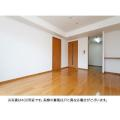
\includegraphics[width=\textwidth]{chapters/plots/ranked_properties/ceiling/top_k/livingroom/42_b5_ed74c84785b3e9a33bf6a54ee3c1_0006.jpg}
        \caption*{High Ceiling - Living Room 2}
    \end{subfigure}
    
    \begin{subfigure}[b]{0.22\textwidth}
        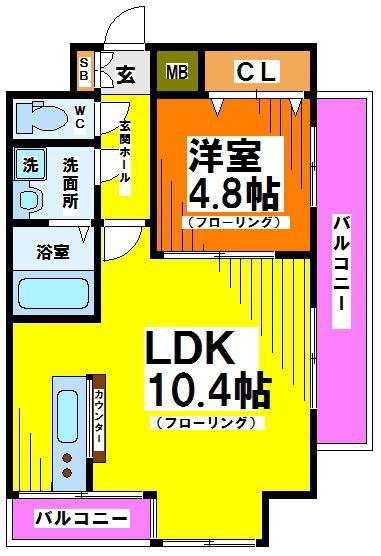
\includegraphics[width=\textwidth]{chapters/plots/ranked_properties/ceiling/bottom_k/floorplan/07_fc_1e6d0c336d417e2af325358cfa1e_0002.jpg}
        \caption*{Low Ceiling - Floorplan 1}
    \end{subfigure}
    \begin{subfigure}[b]{0.22\textwidth}
        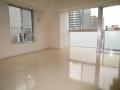
\includegraphics[width=\textwidth]{chapters/plots/ranked_properties/ceiling/bottom_k/livingroom/07_fc_1e6d0c336d417e2af325358cfa1e_0005.jpg}
        \caption*{Low Ceiling - Living Room 1}
    \end{subfigure}
    \begin{subfigure}[b]{0.22\textwidth}
        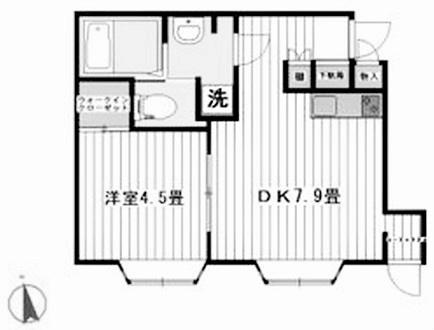
\includegraphics[width=\textwidth]{chapters/plots/ranked_properties/ceiling/bottom_k/floorplan/0f_c8_7478b324cc7c44b35a3b9e1dd340_0002.jpg}
        \caption*{Low Ceiling - Floorplan 2}
    \end{subfigure}
    \begin{subfigure}[b]{0.22\textwidth}
        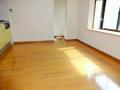
\includegraphics[width=\textwidth]{chapters/plots/ranked_properties/ceiling/bottom_k/livingroom/0f_c8_7478b324cc7c44b35a3b9e1dd340_0005.jpg}
        \caption*{Low Ceiling - Living Room 2}
    \end{subfigure}
    \caption{Comparison of properties with high (top row) and low (bottom row) ceiling visibility ratios, illustrating the impact of vertical space design with both floor plans and corresponding living room images.}
    \label{fig:ceiling_comparison}
\end{figure}

\subsubsection{Floor Visibility}

\begin{figure}[H]
    \centering
    \begin{subfigure}[b]{0.22\textwidth}
        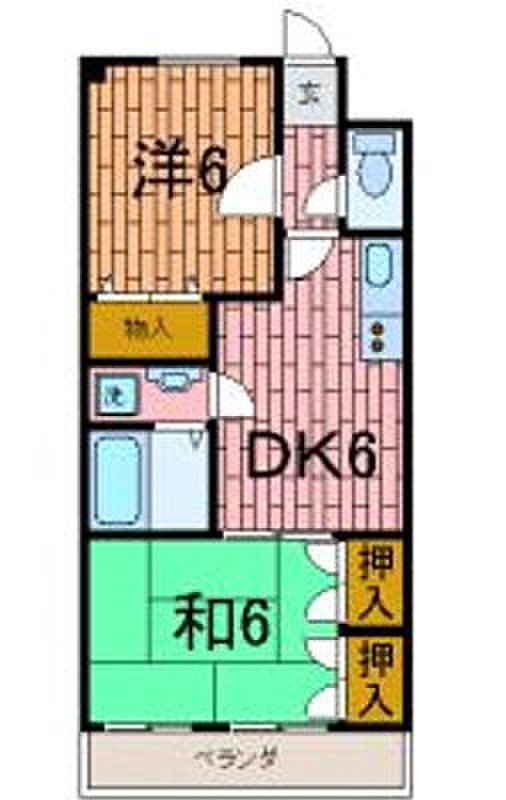
\includegraphics[width=\textwidth]{chapters/plots/ranked_properties/floor/top_k/floorplan/10_d3_a124059139452f4258761327706c_0001.jpg}
        \caption*{High Floor - Floorplan 1}
    \end{subfigure}
    \begin{subfigure}[b]{0.22\textwidth}
        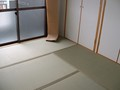
\includegraphics[width=\textwidth]{chapters/plots/ranked_properties/floor/top_k/livingroom/10_d3_a124059139452f4258761327706c_0006.jpg}
        \caption*{High Floor - Living Room 1}
    \end{subfigure}
    \begin{subfigure}[b]{0.22\textwidth}
        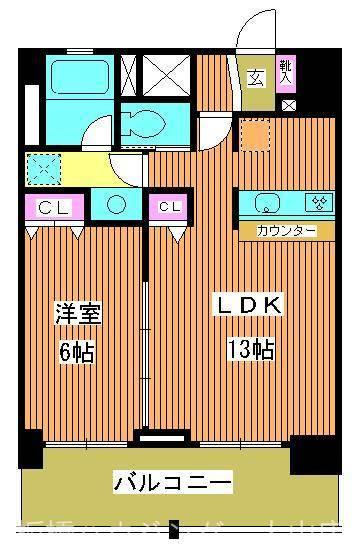
\includegraphics[width=\textwidth]{chapters/plots/ranked_properties/floor/top_k/floorplan/13_4b_f382d831061446a50e8ccdc147ac_0002.jpg}
        \caption*{High Floor - Floorplan 2}
    \end{subfigure}
    \begin{subfigure}[b]{0.22\textwidth}
        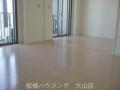
\includegraphics[width=\textwidth]{chapters/plots/ranked_properties/floor/top_k/livingroom/13_4b_f382d831061446a50e8ccdc147ac_0003.jpg}
        \caption*{High Floor - Living Room 2}
    \end{subfigure}
    
    \begin{subfigure}[b]{0.22\textwidth}
        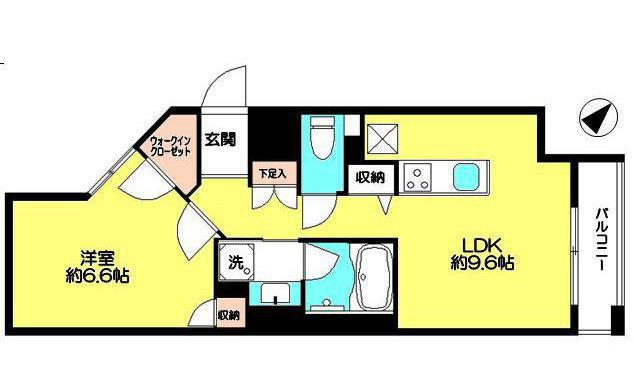
\includegraphics[width=\textwidth]{chapters/plots/ranked_properties/floor/bottom_k/floorplan/07_eb_abc39f577becdc073052e0ee4590_0002.jpg}
        \caption*{Low Floor - Floorplan 1}
    \end{subfigure}
    \begin{subfigure}[b]{0.22\textwidth}
        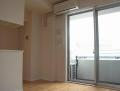
\includegraphics[width=\textwidth]{chapters/plots/ranked_properties/floor/bottom_k/livingroom/07_eb_abc39f577becdc073052e0ee4590_0003.jpg}
        \caption*{Low Floor - Living Room 1}
    \end{subfigure}
    \begin{subfigure}[b]{0.22\textwidth}
        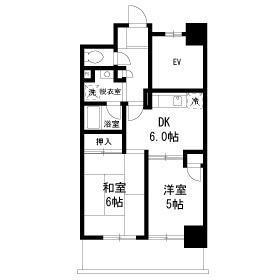
\includegraphics[width=\textwidth]{chapters/plots/ranked_properties/floor/bottom_k/floorplan/cf_d7_25599f305dda3c420563eec70042_0001.jpg}
        \caption*{Low Floor - Floorplan 2}
    \end{subfigure}
    \begin{subfigure}[b]{0.22\textwidth}
        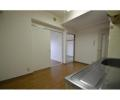
\includegraphics[width=\textwidth]{chapters/plots/ranked_properties/floor/bottom_k/livingroom/cf_d7_25599f305dda3c420563eec70042_0003.jpg}
        \caption*{Low Floor - Living Room 2}
    \end{subfigure}
    \caption{Comparison of properties with high (top row) and low (bottom row) floor visibility ratios, showing the impact of floor area visibility on spatial perception with both floor plans and corresponding living room images.}
    \label{fig:floor_comparison}
\end{figure}

\subsubsection{Wall Visibility}

\begin{figure}[H]
    \centering
    \begin{subfigure}[b]{0.22\textwidth}
        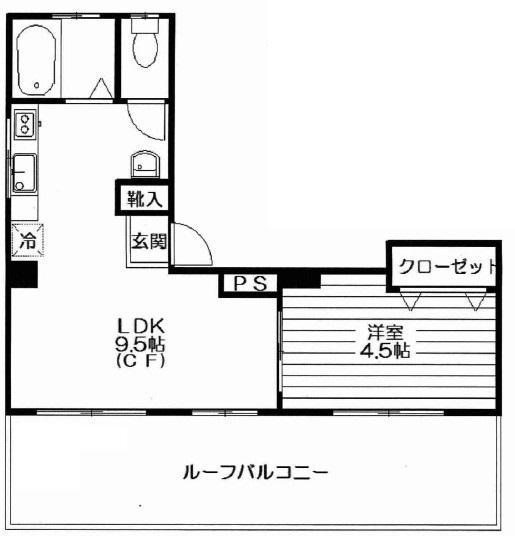
\includegraphics[width=\textwidth]{chapters/plots/ranked_properties/wall/top_k/floorplan/dd_cd_5ede679e5528561ed24c8b000140_0002.jpg}
        \caption*{High Wall - Floorplan 1}
    \end{subfigure}
    \begin{subfigure}[b]{0.22\textwidth}
        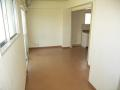
\includegraphics[width=\textwidth]{chapters/plots/ranked_properties/wall/top_k/livingroom/dd_cd_5ede679e5528561ed24c8b000140_0005.jpg}
        \caption*{High Wall - Living Room 1}
    \end{subfigure}
    \begin{subfigure}[b]{0.22\textwidth}
        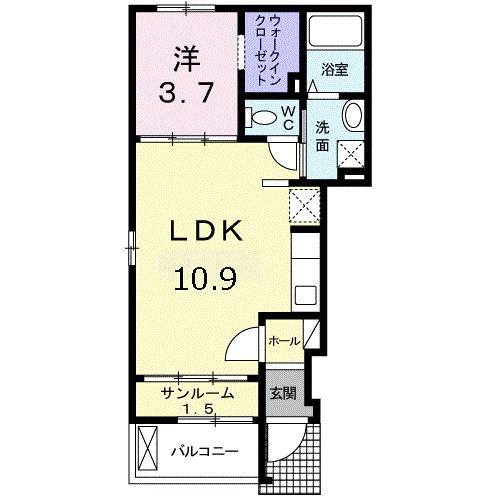
\includegraphics[width=\textwidth]{chapters/plots/ranked_properties/wall/top_k/floorplan/1c_09_71803d8a85fbd9867bb8087d58a6_0002.jpg}
        \caption*{High Wall - Floorplan 2}
    \end{subfigure}
    \begin{subfigure}[b]{0.22\textwidth}
        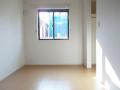
\includegraphics[width=\textwidth]{chapters/plots/ranked_properties/wall/top_k/livingroom/1c_09_71803d8a85fbd9867bb8087d58a6_0005.jpg}
        \caption*{High Wall - Living Room 2}
    \end{subfigure}
    
    \begin{subfigure}[b]{0.22\textwidth}
        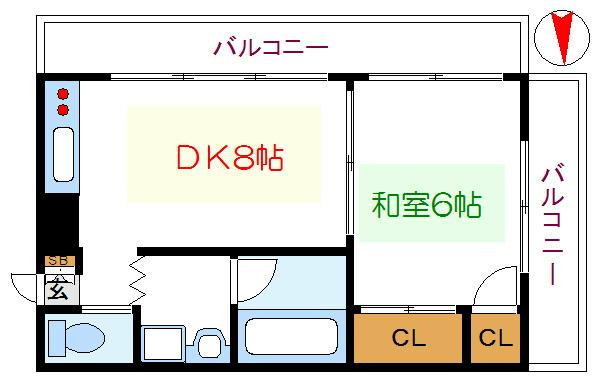
\includegraphics[width=\textwidth]{chapters/plots/ranked_properties/wall/bottom_k/floorplan/0b_a5_e5ed745128fae63c4e99a7642c90_0002.jpg}
        \caption*{Low Wall - Floorplan 1}
    \end{subfigure}
    \begin{subfigure}[b]{0.22\textwidth}
        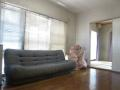
\includegraphics[width=\textwidth]{chapters/plots/ranked_properties/wall/bottom_k/livingroom/0b_a5_e5ed745128fae63c4e99a7642c90_0005.jpg}
        \caption*{Low Wall - Living Room 1}
    \end{subfigure}
    \begin{subfigure}[b]{0.22\textwidth}
        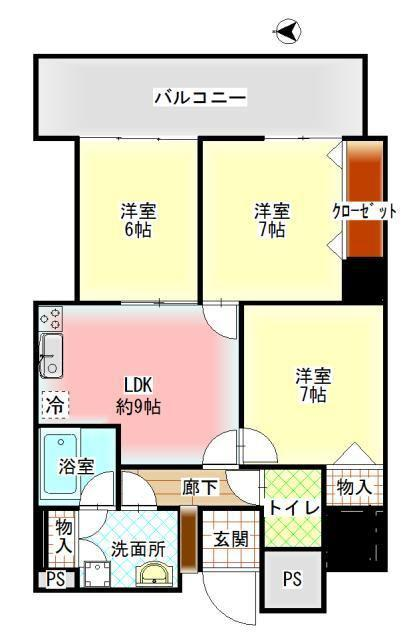
\includegraphics[width=\textwidth]{chapters/plots/ranked_properties/wall/bottom_k/floorplan/40_e1_224ee89fc5abd1a6d916acb5db6f_0001.jpg}
        \caption*{Low Wall - Floorplan 2}
    \end{subfigure}
    \begin{subfigure}[b]{0.22\textwidth}
        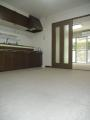
\includegraphics[width=\textwidth]{chapters/plots/ranked_properties/wall/bottom_k/livingroom/40_e1_224ee89fc5abd1a6d916acb5db6f_0003.jpg}
        \caption*{Low Wall - Living Room 2}
    \end{subfigure}
    \caption{Comparison of properties with high (top row) and low (bottom row) wall visibility ratios, demonstrating the relationship between architectural complexity and wall exposure with both floor plans and corresponding living room images.}
    \label{fig:wall_comparison}
\end{figure}

\subsection{Combined Indicator Analysis}

\subsubsection{High visibility values with Low Window Ratio}

\begin{figure}[H]
    \centering
    \begin{subfigure}[b]{0.22\textwidth}
        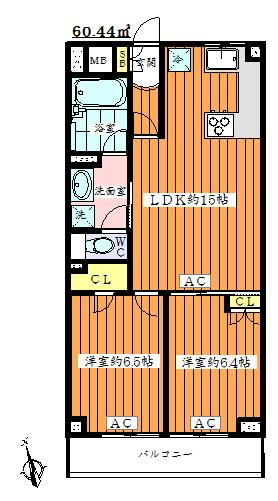
\includegraphics[width=\textwidth]{chapters/plots/ranked_properties/high_mean_value_raw_all_low_windowpane/floorplan/50_ce_c18887f633d07821c92f509fc6e5_0001.jpg}
        \caption*{High visibility Low Window - Floorplan 1}
    \end{subfigure}
    \begin{subfigure}[b]{0.22\textwidth}
        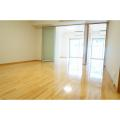
\includegraphics[width=\textwidth]{chapters/plots/ranked_properties/high_mean_value_raw_all_low_windowpane/interior/50_ce_c18887f633d07821c92f509fc6e5_0003.jpg}
        \caption*{High visibility Low Window - Interior 1}
    \end{subfigure}
    \begin{subfigure}[b]{0.22\textwidth}
        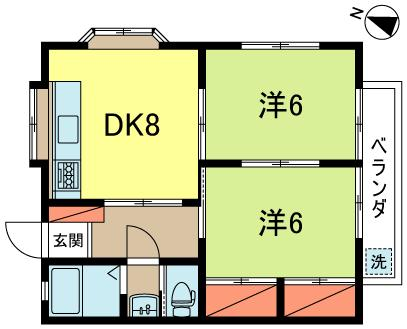
\includegraphics[width=\textwidth]{chapters/plots/ranked_properties/high_mean_value_raw_all_low_windowpane/floorplan/52_a8_5d745c13c0ce8ef62ced75cdacb2_0002.jpg}
        \caption*{High visibility Low Window - Floorplan 2}
    \end{subfigure}
    \begin{subfigure}[b]{0.22\textwidth}
        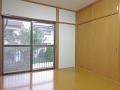
\includegraphics[width=\textwidth]{chapters/plots/ranked_properties/high_mean_value_raw_all_low_windowpane/interior/52_a8_5d745c13c0ce8ef62ced75cdacb2_0005.jpg}
        \caption*{High visibility Low Window - Interior 2}
    \end{subfigure}
    \caption{Properties with high mean visibility values but low window ratios, demonstrating 2D openness achieved through layout design rather than glazing with both floor plans and corresponding interior images.}
    \label{fig:high_vga_low_window}
\end{figure}

\subsubsection{High visibility values with High Window Ratio}

\begin{figure}[H]
    \centering
    \begin{subfigure}[b]{0.22\textwidth}
        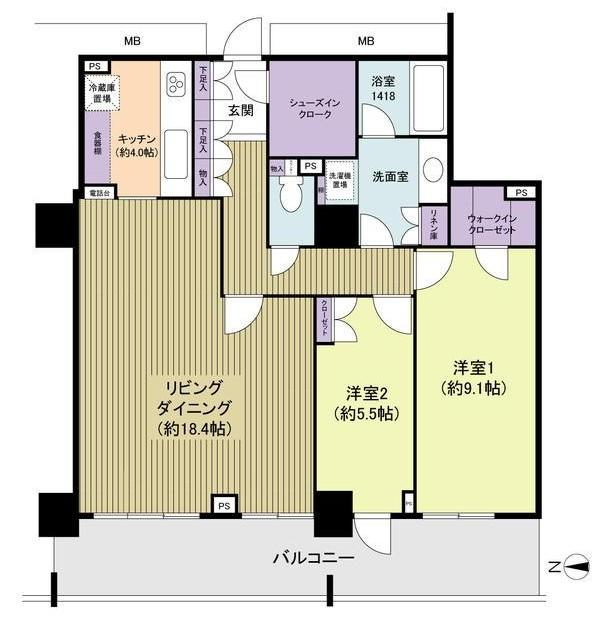
\includegraphics[width=\textwidth]{chapters/plots/ranked_properties/high_mean_value_raw_all_high_windowpane/floorplan/12_b6_10d6ee0bc39bfc0c964529e8a0f3_0002.jpg}
        \caption*{High visibility High Window - Floorplan 1}
    \end{subfigure}
    \begin{subfigure}[b]{0.22\textwidth}
        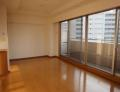
\includegraphics[width=\textwidth]{chapters/plots/ranked_properties/high_mean_value_raw_all_high_windowpane/interior/12_b6_10d6ee0bc39bfc0c964529e8a0f3_0008.jpg}
        \caption*{High visibility High Window - Interior 1}
    \end{subfigure}
    \begin{subfigure}[b]{0.22\textwidth}
        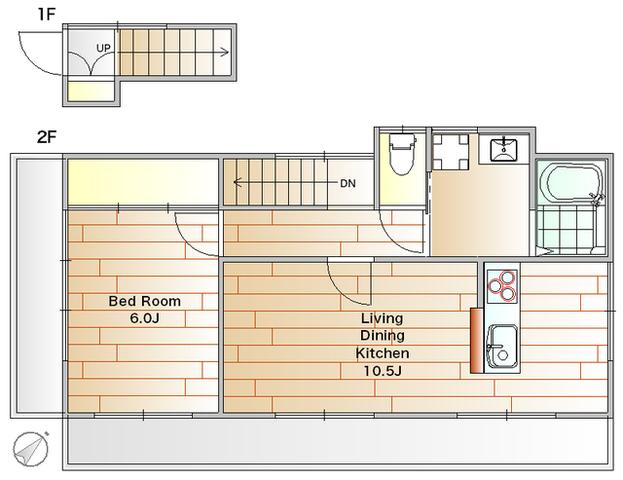
\includegraphics[width=\textwidth]{chapters/plots/ranked_properties/high_mean_value_raw_all_high_windowpane/floorplan/38_0d_4e9b32327ff72f5bb8180cc2350d_0003.jpg}
        \caption*{High visibility High Window - Floorplan 2}
    \end{subfigure}
    \begin{subfigure}[b]{0.22\textwidth}
        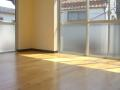
\includegraphics[width=\textwidth]{chapters/plots/ranked_properties/high_mean_value_raw_all_high_windowpane/interior/38_0d_4e9b32327ff72f5bb8180cc2350d_0007.jpg}
        \caption*{High visibility High Window - Interior 2}
    \end{subfigure}
    \caption{Properties with both high mean visibility values and high window ratios, representing optimal combinations of 2D and 3D openness characteristics with both floor plans and corresponding interior images.}
    \label{fig:high_vga_high_window}
\end{figure}

\subsubsection{Low visibility values with High Window Ratio}

\begin{figure}[H]
    \centering
    \begin{subfigure}[b]{0.22\textwidth}
        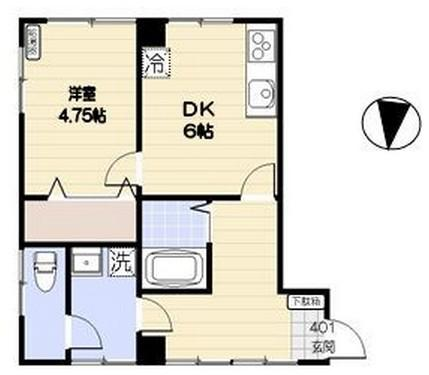
\includegraphics[width=\textwidth]{chapters/plots/ranked_properties/low_mean_value_raw_all_high_windowpane/floorplan/0f_60_4389dc3851937a3a3e78da1e1e5e_0002.jpg}
        \caption*{Low visibility High Window - Floorplan 1}
    \end{subfigure}
    \begin{subfigure}[b]{0.22\textwidth}
        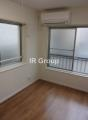
\includegraphics[width=\textwidth]{chapters/plots/ranked_properties/low_mean_value_raw_all_high_windowpane/interior/0f_60_4389dc3851937a3a3e78da1e1e5e_0003.jpg}
        \caption*{Low visibility High Window - Interior 1}
    \end{subfigure}
    \begin{subfigure}[b]{0.22\textwidth}
        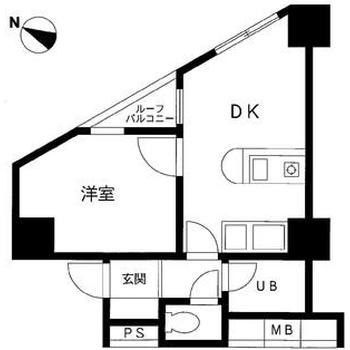
\includegraphics[width=\textwidth]{chapters/plots/ranked_properties/low_mean_value_raw_all_high_windowpane/floorplan/2b_af_6cbd477454741678ed92a966fa38_0002.jpg}
        \caption*{Low visibility High Window - Floorplan 2}
    \end{subfigure}
    \begin{subfigure}[b]{0.22\textwidth}
        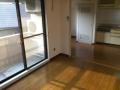
\includegraphics[width=\textwidth]{chapters/plots/ranked_properties/low_mean_value_raw_all_high_windowpane/interior/2b_af_6cbd477454741678ed92a966fa38_0003.jpg}
        \caption*{Low visibility High Window - Interior 2}
    \end{subfigure}
    \caption{Properties with low mean visibility values but high window ratios, showing how extensive glazing can provide openness despite compartmentalized layouts with both floor plans and corresponding interior images.}
    \label{fig:low_vga_high_window}
\end{figure}

\subsubsection{Low visibility values with Low Window Ratio}

\begin{figure}[H]
    \centering
    \begin{subfigure}[b]{0.22\textwidth}
        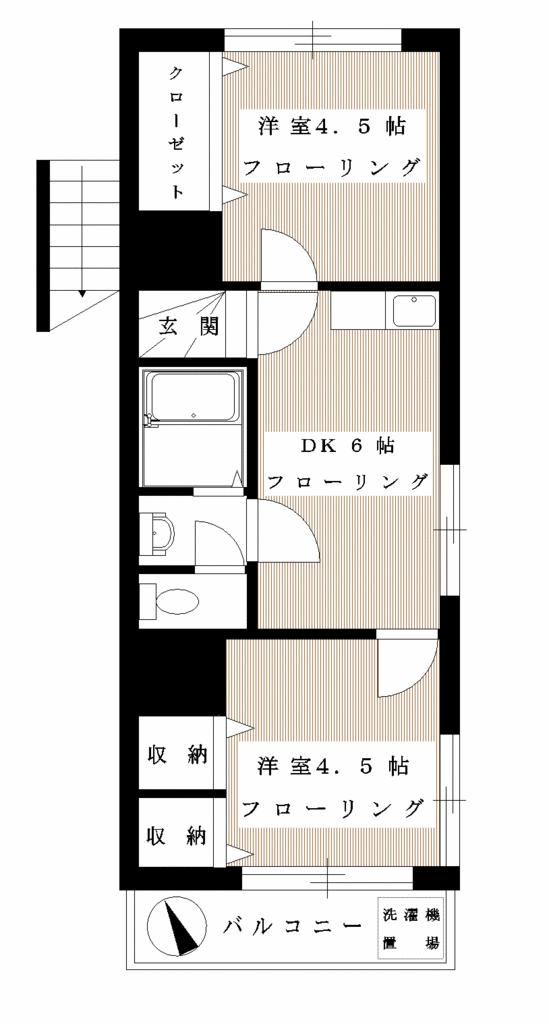
\includegraphics[width=\textwidth]{chapters/plots/ranked_properties/low_mean_value_raw_all_low_windowpane/floorplan/50_4f_f64209392200a7733dd015ec748f_0002.jpg}
        \caption*{Low visibility Low Window - Floorplan 1}
    \end{subfigure}
    \begin{subfigure}[b]{0.22\textwidth}
        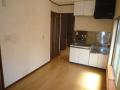
\includegraphics[width=\textwidth]{chapters/plots/ranked_properties/low_mean_value_raw_all_low_windowpane/interior/50_4f_f64209392200a7733dd015ec748f_0003.jpg}
        \caption*{Low visibility Low Window - Interior 1}
    \end{subfigure}
    \begin{subfigure}[b]{0.22\textwidth}
        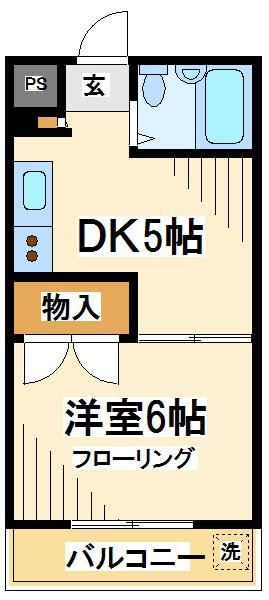
\includegraphics[width=\textwidth]{chapters/plots/ranked_properties/low_mean_value_raw_all_low_windowpane/floorplan/50_9d_20303e80370289d37407f96cf27f_0002.jpg}
        \caption*{Low visibility Low Window - Floorplan 2}
    \end{subfigure}
    \begin{subfigure}[b]{0.22\textwidth}
        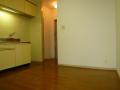
\includegraphics[width=\textwidth]{chapters/plots/ranked_properties/low_mean_value_raw_all_low_windowpane/interior/50_9d_20303e80370289d37407f96cf27f_0005.jpg}
        \caption*{Low visibility Low Window - Interior 2}
    \end{subfigure}
    \caption{Properties with both low mean visibility values and low window ratios, representing the most enclosed characteristics with emphasis on privacy and separation with both floor plans and corresponding interior images.}
    \label{fig:low_vga_low_window}
\end{figure}
